\documentclass{article}
\usepackage[top=1cm,bottom=1cm,left=2cm,right=2cm]{geometry}
\usepackage{amsmath}
\usepackage{graphicx}
\title{Advanced Computational Science Assignment 2}
\author{Liam O'Sullivan --- 10309537}
\date{\today}
\pagestyle{empty}


\newcommand{\uhalf}{u^{n+1/2}}
\begin{document}
\maketitle
\thispagestyle{empty}

\section*{The Alternating Direction Implicit Method}
The Alternative Direction Implicit (ADI) method is an implicit numerical method similar to the
Crank-Nicholson method. It is given by
\begin{equation}
  (1 - \frac{\alpha_x}{2}\delta^2_x)(1 - \frac{\alpha_y}{2}\delta^2_y) u_{i,j}^{n+1} = 
  (1 + \frac{\alpha_x}{2}\delta^2_x)(1 + \frac{\alpha_y}{2}\delta^2_y) u_{i,j}^n
\end{equation}
where $\alpha_\gamma = \frac{\tau}{h_\gamma^2}$.
Interestingly, this method can be broken into two steps:
$$
  (1 - \frac{\alpha_x}{2}\delta^2_x)\uhalf_{i,j} = 
  (1 + \frac{\alpha_y}{2}\delta^2_y) u_{i,j}^n
$$
$$
  (1 - \frac{\alpha_y}{2}\delta^2_y)u_{i,j}^{n+1} = 
  (1 + \frac{\alpha_x}{2}\delta^2_x) \uhalf_{i,j}
$$
where the $x$-derivative is taken implicitly in the first step, and the $y$-derivative taken implicitly
in the second.

Expanding the first expression above gives
$$
  - \frac{\alpha_x}{2}\uhalf_{i-1,j} + (1+\alpha_x)\uhalf_{i,j} - \frac{\alpha_x}{2} = 
  \frac{\alpha_y}{2}u^n_{i,j-1} + (1-\alpha_y)u^n_{i,j} - \frac{\alpha_y}{2}u^n_{i,j+1}
$$
where the right side can be computed explicitly.
We can write this in matrix form,
$$
  \left( \begin{array}{cccccc}
  1+\alpha & -\frac{\alpha}{2} & 0 & \cdot & \cdot& 0 \\
  -\frac{\alpha}{2} & 1+\alpha & -\frac{\alpha}{2} & 0 & \cdot & \cdot \\
  0 & -\frac{\alpha}{2} & 1+\alpha & -\frac{\alpha}{2} & \cdot & \cdot\\
  \cdot & \cdot & \cdot & \cdot & \cdot& \cdot\\
  \cdot & \cdot & \cdot & \cdot & \cdot& \cdot\\
  0 & \cdot& \cdot& \cdot &  -\frac{\alpha}{2} & 1+\alpha \\ \end{array} \right)
  \left( \begin{array}{c}
  \uhalf_{0,j} \\
  \uhalf_{1,j} \\
  \cdot \\
  \cdot \\
  \uhalf_{n_x,j} \\ \end{array} \right)
  =
  \left( \begin{array}{c}
  d^n_{0,j} \\
  d^n_{1,j} \\
  \cdot \\
  \cdot \\
  d^n_{n_x,j} \\ \end{array} \right)
$$
where $d^n_{i,j}$ is the explicitly computed part of the previous expression.
As this matrix is clearly diagonally dominant and tridiagonal, we can use the Thomas Algorithm to solve
for the unknown $\uhalf$.
This is done by bringing the matrix into upper triangular form. As an example, the matrix equation
$$
  \left( \begin{array}{cccccc}
  b_1 & -c_1 & 0 & \cdot & \cdot& 0 \\
  -a_2 & b_2 & -c_2 & 0 & \cdot & \cdot \\
  0 & -a_3 & b_3 & -c_3 & \cdot & \cdot\\
  \cdot & \cdot & \cdot & \cdot & \cdot& \cdot\\
  \cdot & \cdot & \cdot & \cdot & \cdot& \cdot\\
  0 & \cdot& \cdot& \cdot &  -a_n & b_n \\ \end{array} \right)
  \left( \begin{array}{c}
  u_0 \\
  u_1 \\
  \cdot \\
  \cdot \\
  u_n \\ \end{array} \right)
  =
  \left( \begin{array}{c}
  d_1 \\
  d_2 \\
  \cdot \\
  \cdot \\
  d_n \\ \end{array} \right)
$$
can be transformed into
$$
  \left( \begin{array}{cccccc}
  1& -e_1 & 0 & \cdot & \cdot& 0 \\
  0 & 1 & -e_2 & 0 & \cdot & \cdot \\
  0 & \cdot & 1 & -e_3 & \cdot & \cdot\\
  \cdot & \cdot & \cdot & \cdot & \cdot& \cdot\\
  \cdot & \cdot & \cdot & \cdot & \cdot& \cdot\\
  0 & \cdot& \cdot& \cdot &  \cdot & 1 \\ \end{array} \right)
  \left( \begin{array}{c}
  u_0 \\
  u_1 \\
  \cdot \\
  \cdot \\
  u_n \\ \end{array} \right)
  =
  \left( \begin{array}{c}
  f_1 \\
  f_2 \\
  \cdot \\
  \cdot \\
  f_n \\ \end{array} \right)
$$
with
$$
  e_k = \frac{c_k}{b_k - a_k e_{k-1}}, \hspace{2cm} f_k = \frac{d_k + a_k f_{k-1}}{b_k - a_k e_{k-1}}
$$
As the final line produces an equation of one unknown, it is possible to solve this system through
backwards substitution. This is done for both parts of the ADI method.


\section*{1}
In this section, we are asked simply to write a program which will solve the linear diffusion equation,
\begin{equation}
\frac{\partial u}{\partial t} = \nabla \cdot \nabla u
\end{equation}
in two dimensions, making our equation
\begin{equation}
\frac{\partial u}{\partial t} = \frac{\partial^2 u}{\partial x^2} + \frac{\partial^2 u}{\partial y^2}.
\end{equation}
We are to use the ADI method, described previously.
We are told to solve the equation on a rectangular grid, $x \in [-1,1],~y\in [-1,1]$, with
initial condition $u(x,y,t=0) = (1 - x^2)(1 - y^4) $, and Dirichlet boundary conditions,
$u(-1,y,t) = u(1,y,t) = u(x,-1,t) = u(x,1,t) = 0$.

The program was written in Python 3, and is attached. On the following page are
various snapshots of the function at indicated times. This case was solved on a grid
with spacing $h_x = h_y = 1/200$, and $1000$ time steps.

\begin{figure}
  \centering
  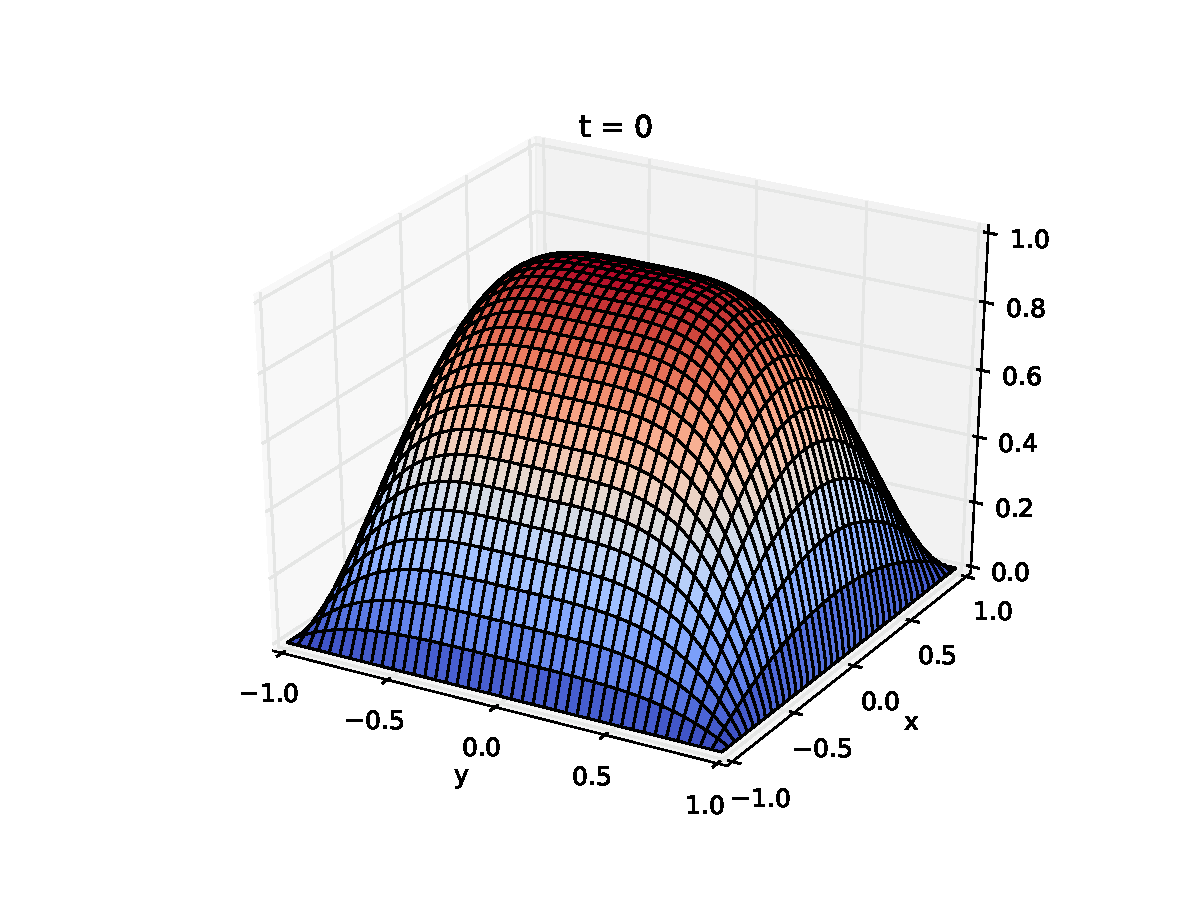
\includegraphics[width=0.5\textwidth]{1/t000.pdf}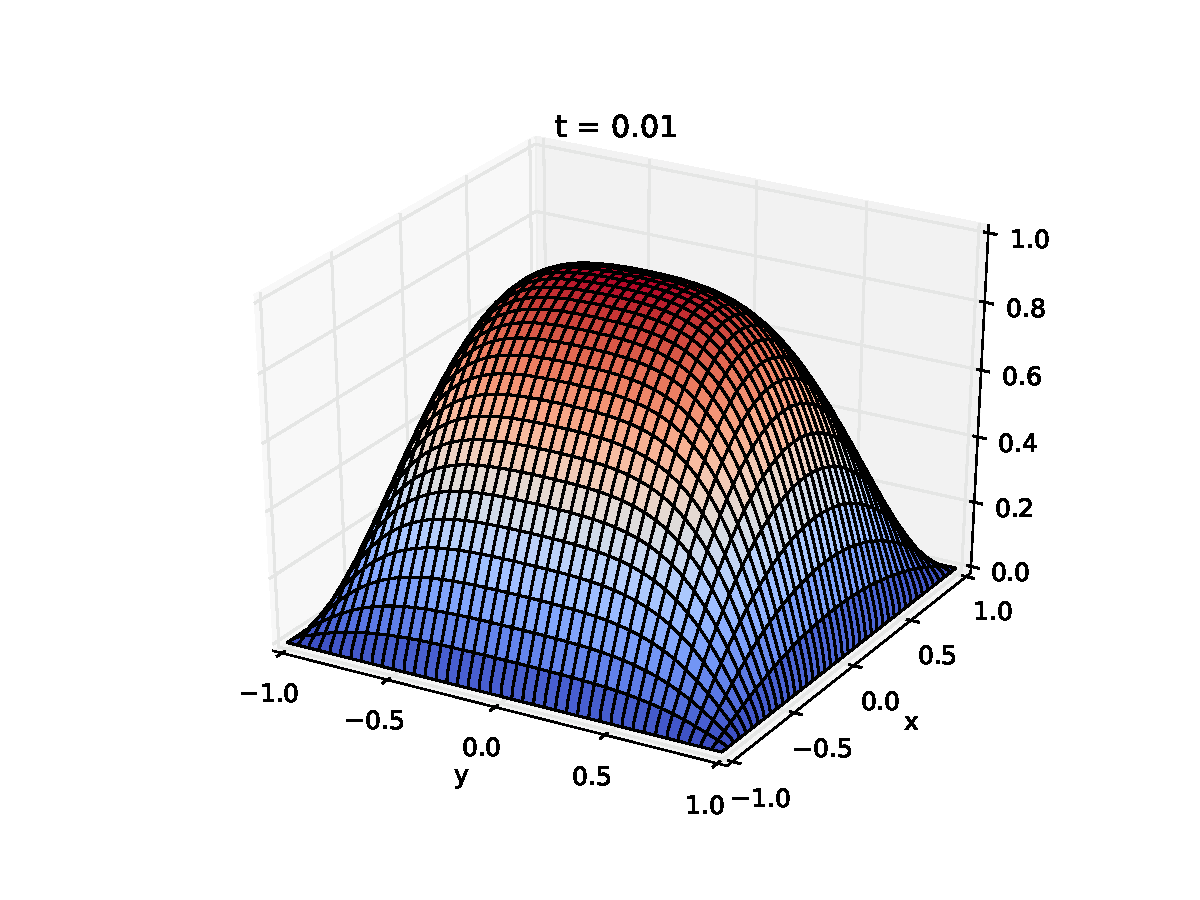
\includegraphics[width=0.5\textwidth]{1/t001.pdf}
  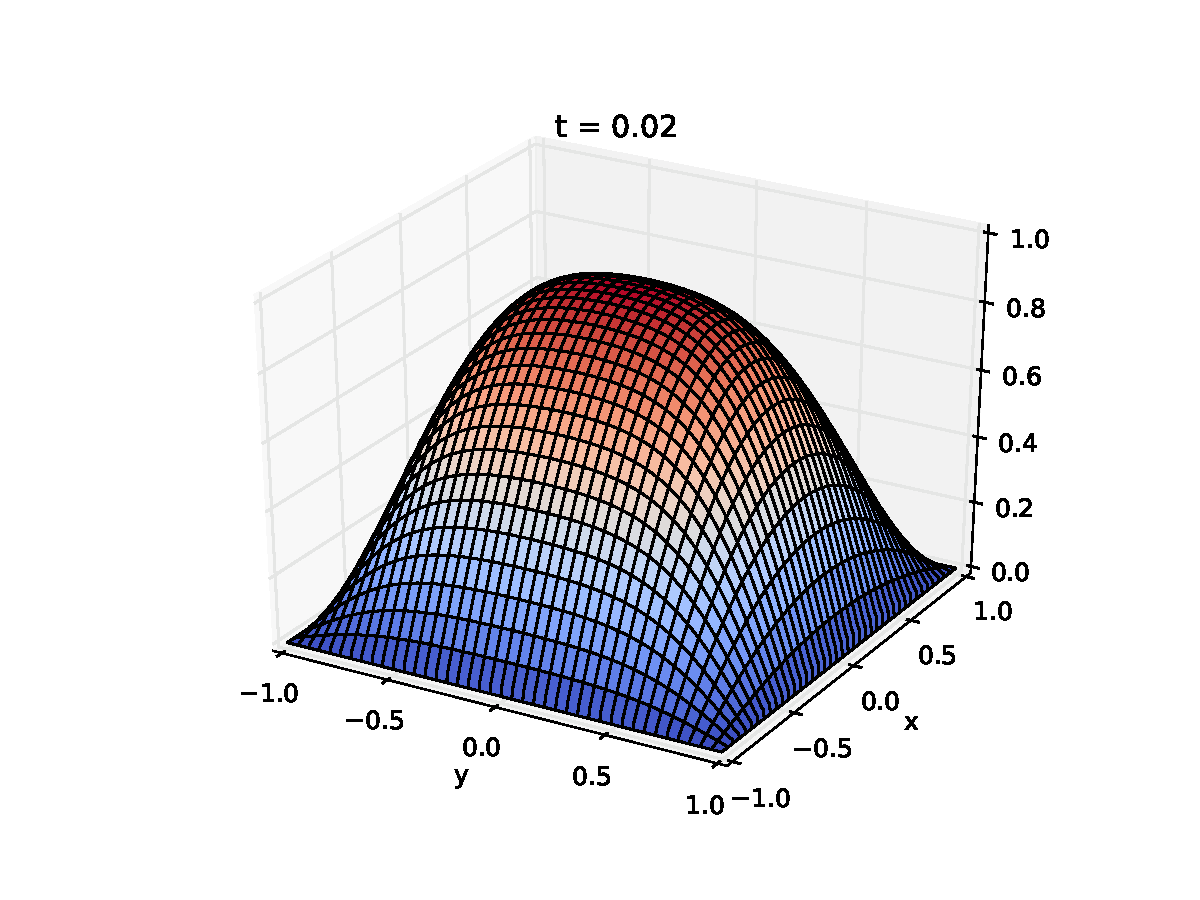
\includegraphics[width=0.5\textwidth]{1/t002.pdf}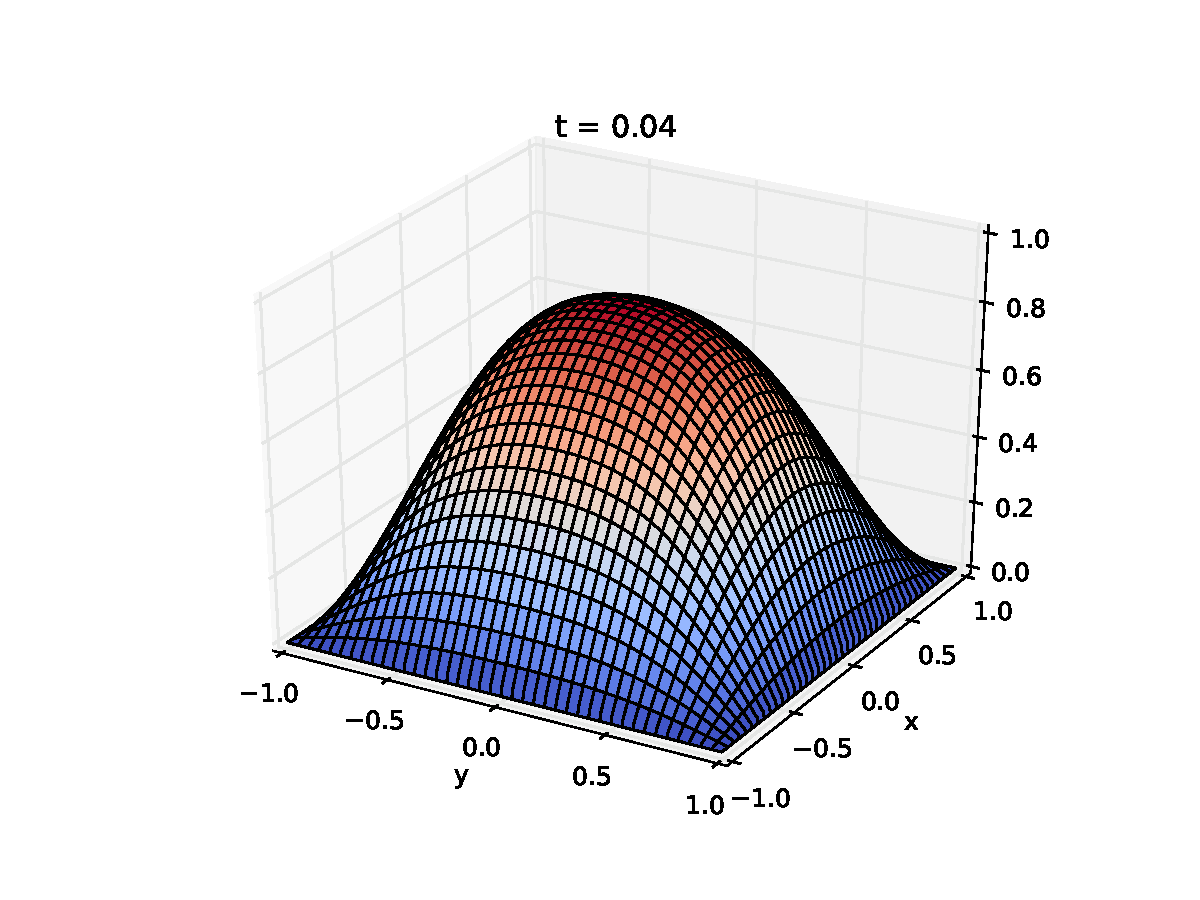
\includegraphics[width=0.5\textwidth]{1/t004.pdf}
  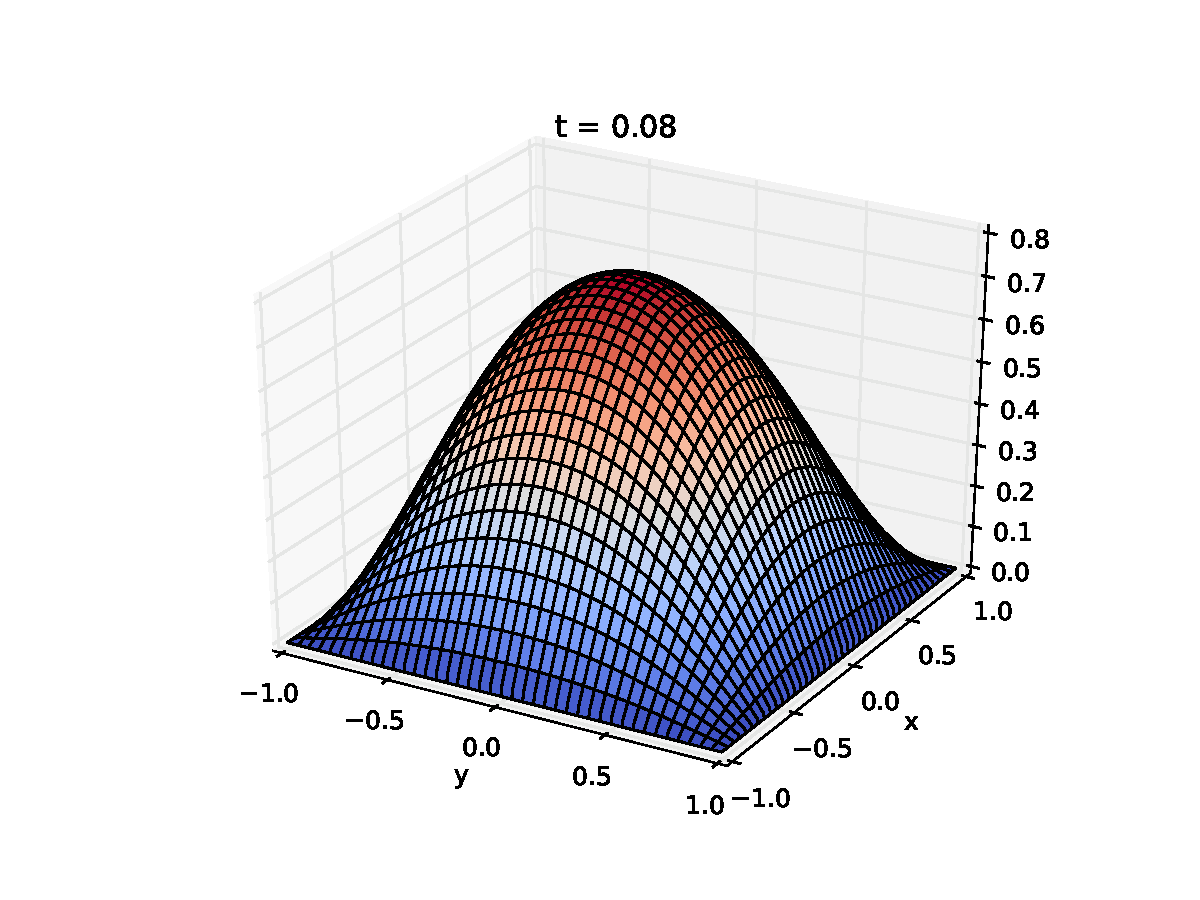
\includegraphics[width=0.5\textwidth]{1/t008.pdf}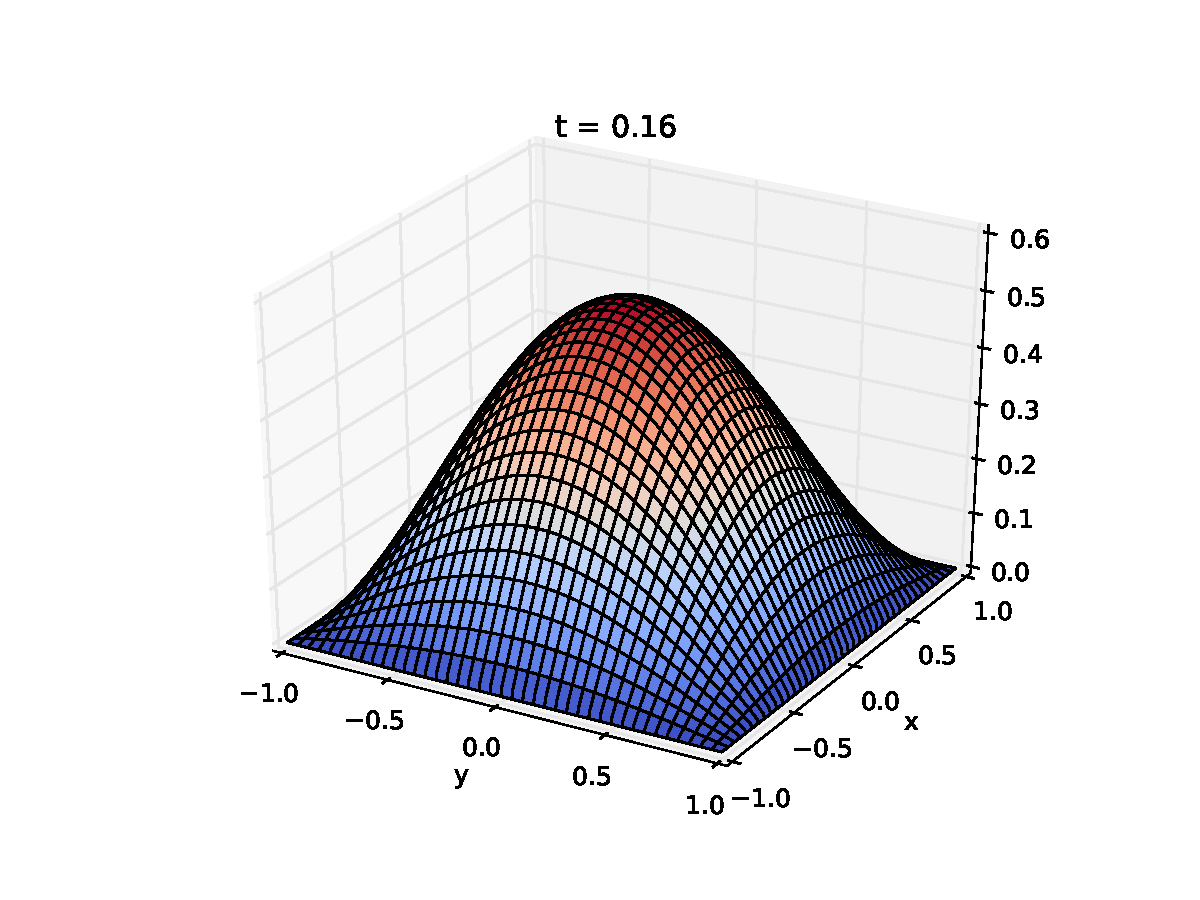
\includegraphics[width=0.5\textwidth]{1/t016.pdf}
  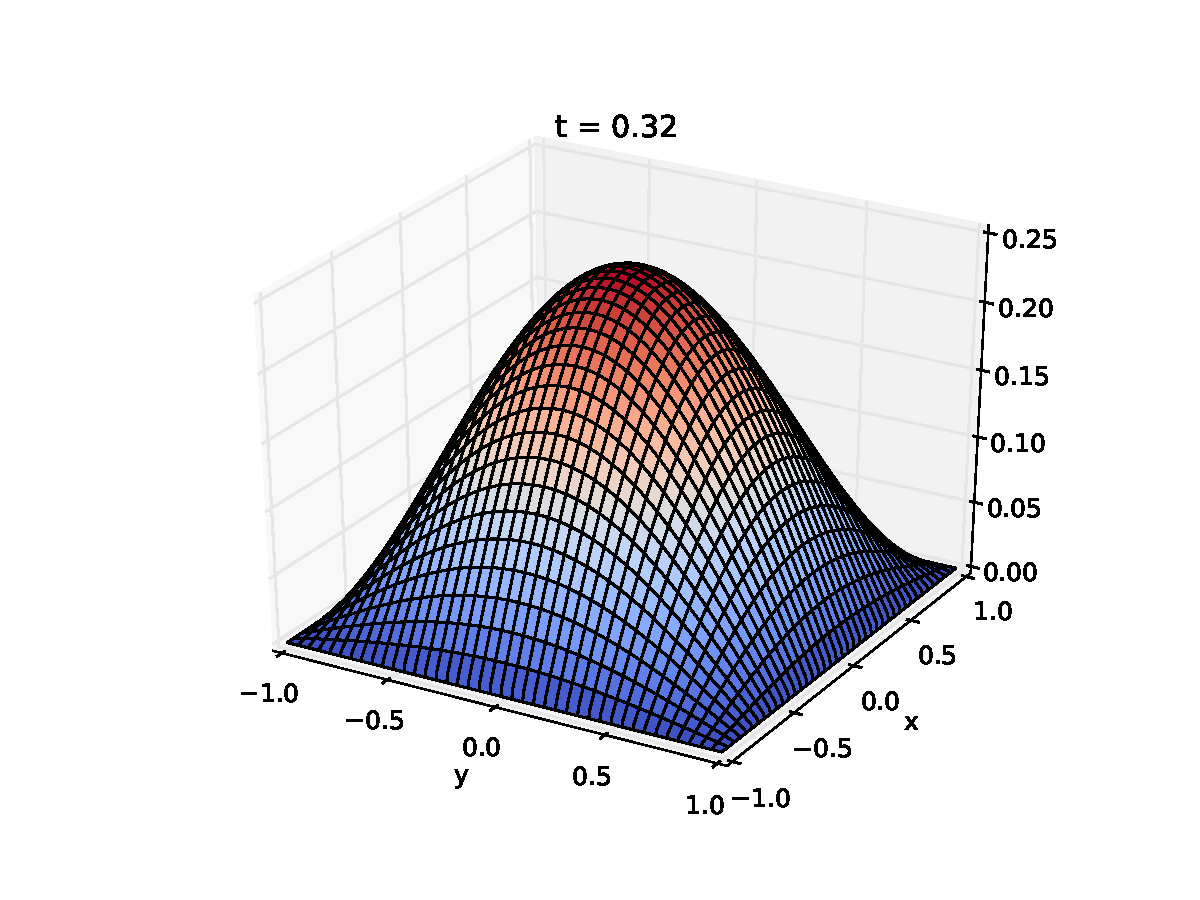
\includegraphics[width=0.5\textwidth]{1/t032.pdf}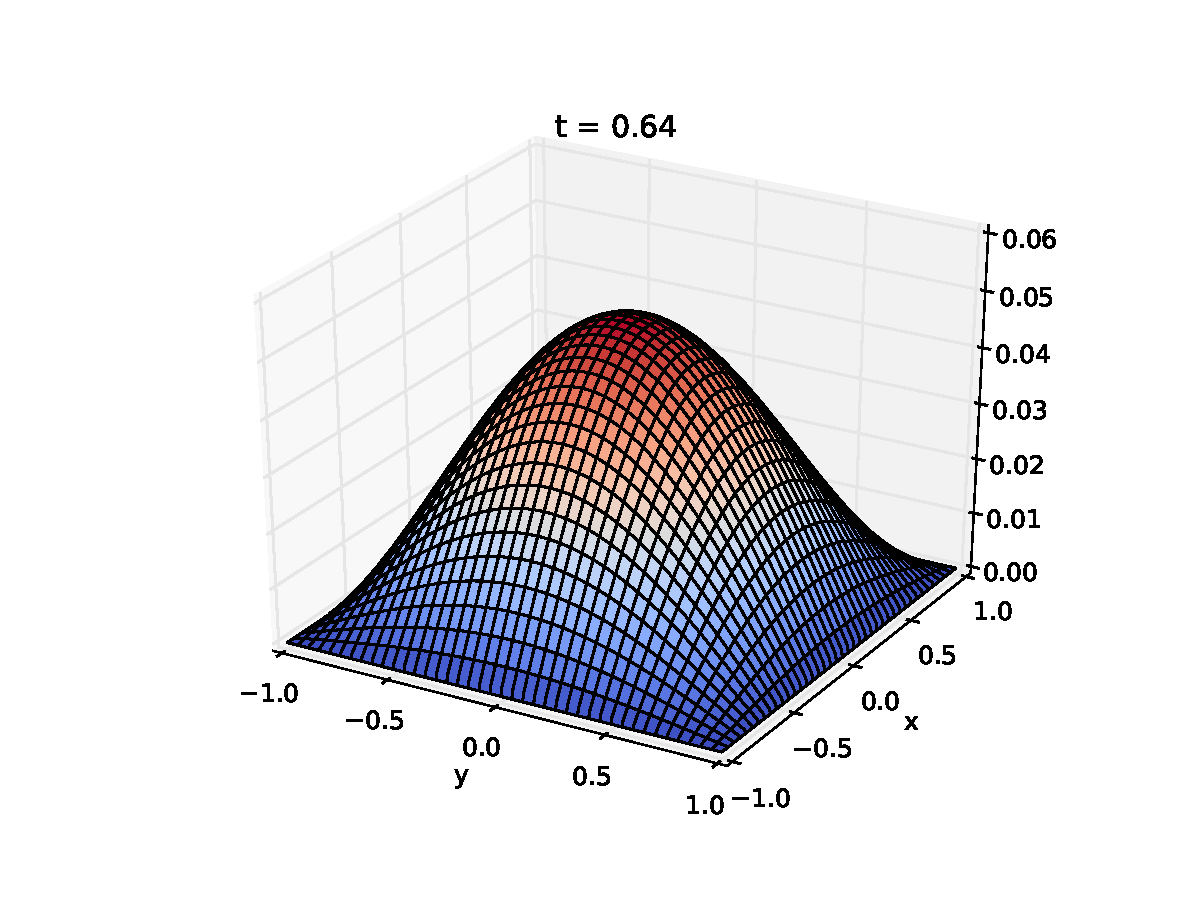
\includegraphics[width=0.5\textwidth]{1/t064.pdf}
\end{figure}

\clearpage
\section*{2}
\subsection*{i}
For this exercise, we are told to take $h_x = h_y = \frac{1}{200}$, and to maximise the number of
time steps in $t \in [0,0.1]$ based on our available memory. In this section, the data for each
time step is saved in one contiguous memory array. The datatype used is a 64-bit float, making
each entry 8 bytes in size. With this, our total memory usage in GB will be 
$$
  M = \frac{8 \times 400^2}{1024^3}n_t
$$
where $n_t$ is the number of time-steps.
Taking $n_t = 1000$ gives just under 1.2GB used by U, which is reasonable on my machine with 2GB
of memory, as this should at no point cause processes to use swap. During the runs, I was
running other programs(Firefox, etc.), making using the entire 2GB undesirable.

\subsection*{ii}
This exercise concerns the $L^2$-norms of the function. The $L^2$-norm is defined as
$$
  | |u(\cdot,t) | |_2 = \sqrt{\int u(x,y,t)^2 dy dx}.
$$
In the code, I have approximated the integral as a sum:
$$
 | | u(\cdot,t) | |_2 \approx \sqrt{ \sum_{i,j} u_{i,j}^2 h_y h_x }
$$

Figure \ref{f:2} shows the evolution of the $L^2$ norms in time for resolutions
$h_0 = 1/200$, $h_1 = 1/100$, $h_2 = 1/50$, with $h_x = h_y = h$.
\begin{figure}
  \centering
  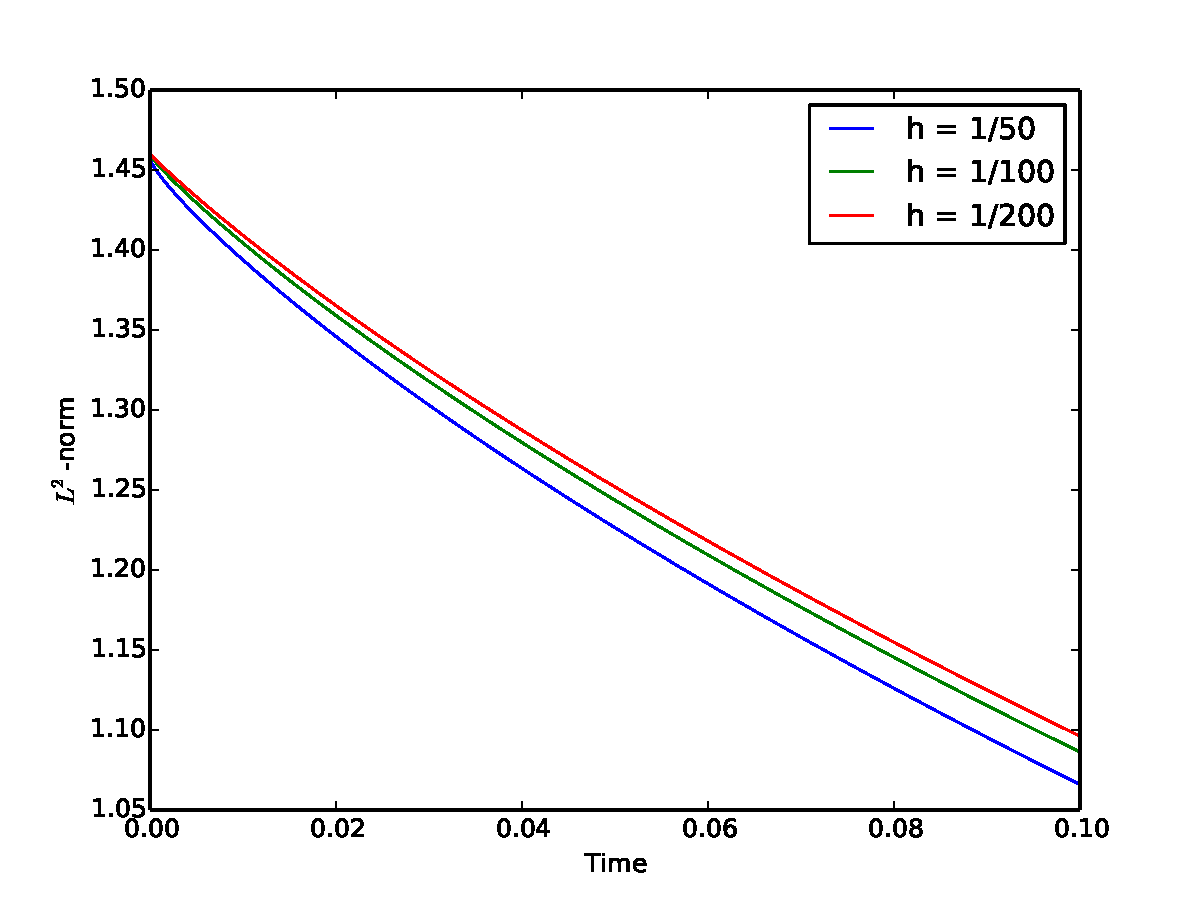
\includegraphics[width=0.7\textwidth]{2/2/plot.pdf}
  \caption{Evolution of $L^2$-norms in time for three resolutions.}
  \label{f:2}
\end{figure}




\subsection*{iii}

\begin{figure}
  \centering
  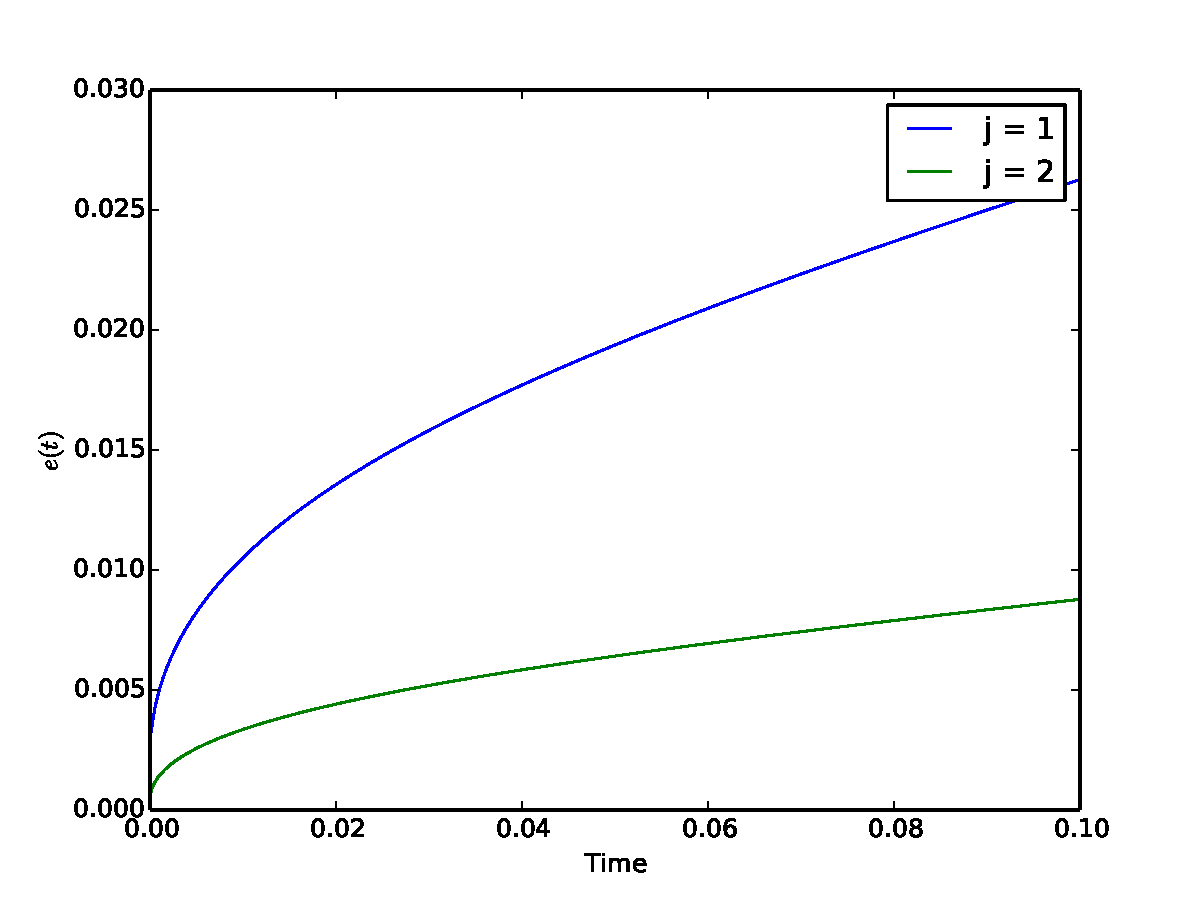
\includegraphics[width=0.7\textwidth]{2/3/plot.pdf}
  \caption{}
  \label{f:3}
\end{figure}

\subsection*{iv}
This section asked to extend the previous resolution study to higher resolutions. To do this, it is recommended
that we do not store the entire array for $u$, but only the amount necessary for computation.
I found that only one array for $u$ and one for $u^{n+1/2}$ are necessary, and the computation
can effectively be done in place. After each run, the $L^2$-norm is computed and assigned into an array
as before. Unfortunately, the runtime for 10 time steps is 300 seconds at the resolution of $h = 1/800$,
making timing and comparing a variety of resolutions arduous. Due to time constraints, $nt=1000$ was used
for this section.


\begin{figure}
  \centering
  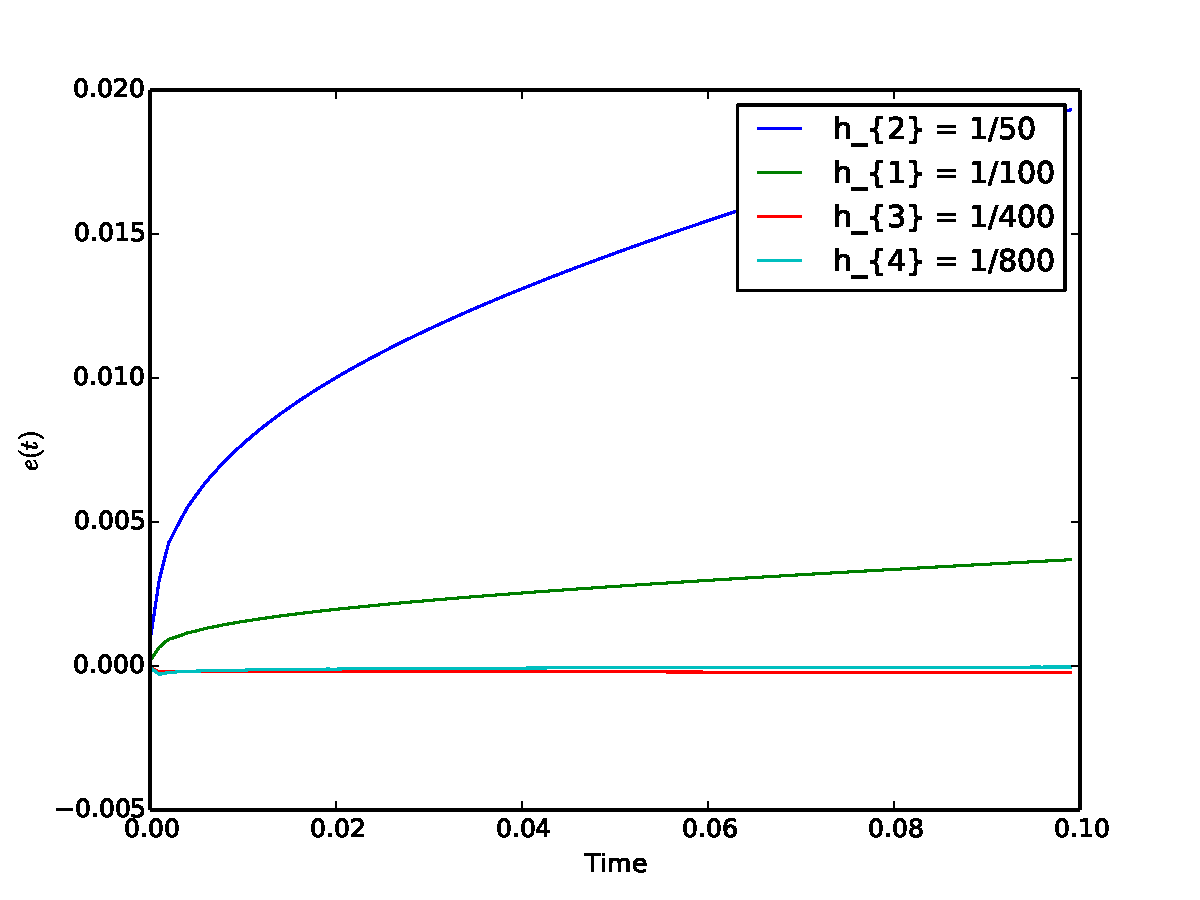
\includegraphics[width=0.7\textwidth]{2/4/plot.pdf}
  \caption{}
  \label{f:41}
\end{figure}

\begin{figure}
  \centering
  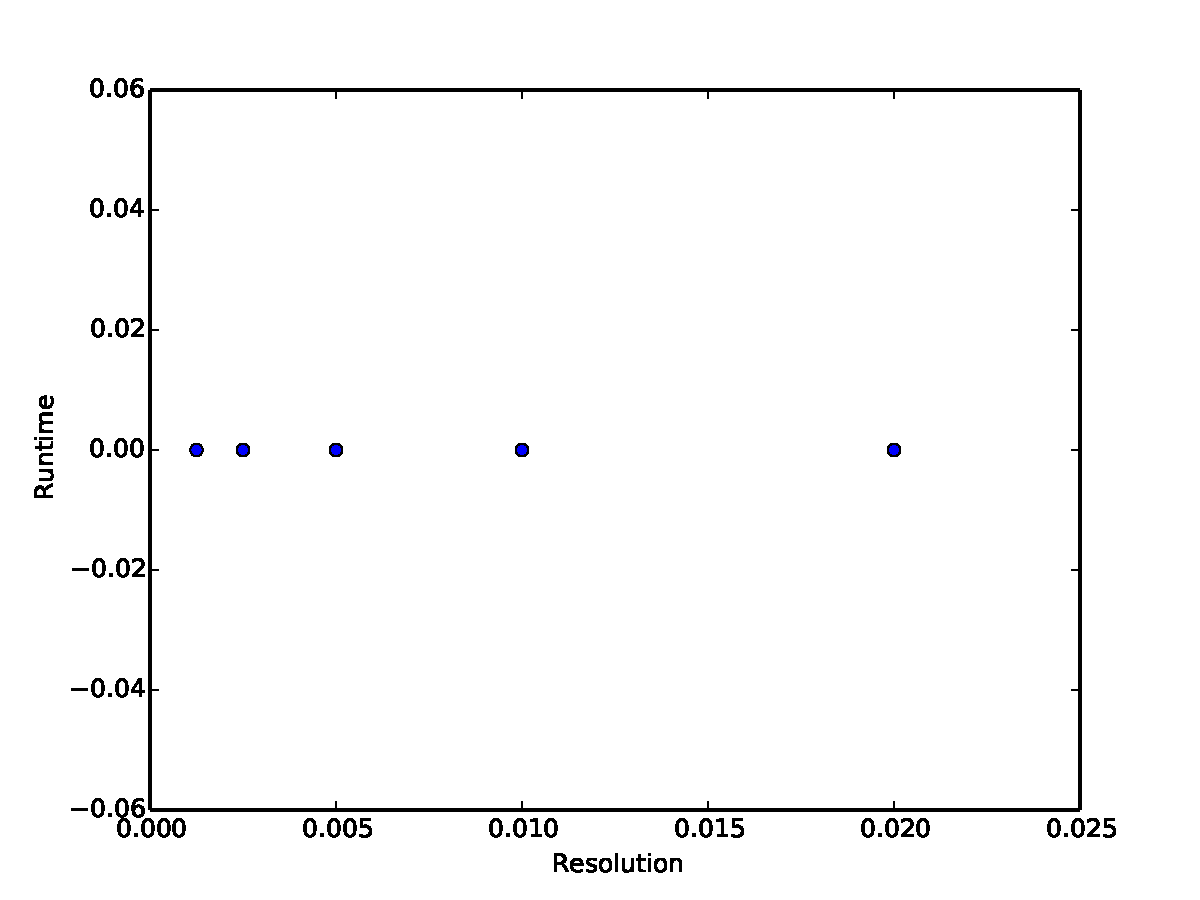
\includegraphics[width=0.7\textwidth]{2/4/resolution.pdf}
  \caption{}
  \label{f:42}
\end{figure}

\end{document}
% vim: spell
% vim: ts=4
% vim: expandtab
